% This version of CVPR template is provided by Ming-Ming Cheng.
% Please leave an issue if you found a bug:
% https://github.com/MCG-NKU/CVPR_Template.

%\documentclass[review]{cvpr}
\documentclass[final]{cvpr}

\usepackage{times}
\usepackage{epsfig}
\usepackage{graphicx}
\graphicspath{{Images/}}
\usepackage{amsmath}
\usepackage{amssymb}

% Include other packages here, before hyperref.

% If you comment hyperref and then uncomment it, you should delete
% egpaper.aux before re-running latex.  (Or just hit 'q' on the first latex
% run, let it finish, and you should be clear).
\usepackage[pagebackref=true,breaklinks=true,colorlinks,bookmarks=false]{hyperref}


\def\cvprPaperID{****} % *** Enter the CVPR Paper ID here
\def\confYear{CVPR 2021}
%\setcounter{page}{4321} % For final version only


\begin{document}

%%%%%%%%% TITLE
\title{Survey on Generative Models}

\author{Steven Walton\\
University of Oregon\\

{\tt\small swalton2@cs.uoregon.edu}
% For a paper whose authors are all at the same institution,
% omit the following lines up until the closing ``}''.
% Additional authors and addresses can be added with ``\and'',
% just like the second author.
% To save space, use either the email address or home page, not both
}

\maketitle


%%%%%%%%% ABSTRACT
\begin{abstract}
Generative models have seen rapid development within the last decade, quickly
progressing from generating fuzzy images to consistently producing images that
are near indistinguishable from real life photos. Besides generating realistic
generative modeling has a wide variety of uses, from image upscaling to
uncovering data augmentation to reduce bias in models. Within this survey we
discuss the different classes of generative models and give an overview of how
they differ and what they can be used for.
\end{abstract}

%%%%%%%%% BODY TEXT
\section{Introduction}
Generative modeling is a subset of machine learning that focuses on generating
new data. This is opposed to the more familiar types of models that classify
data, called a discriminative model. This difference in these is that
discriminative models want to find decision boundaries between a set of data
generative models want to learn how to generate data within that boundary. Or
put more mathematically, a discriminative model learns a conditional probability
given a set of data:  $P(Y=\text{label} | X=\text{data})$.
In turn, a generative model tries to produce new data given a set of data:
$P(x)$. In practice a generative model is only approximating the learned
dataset, so we typically write $p_\theta(\hat{x}) \approx p_{true}(x)$. Here we
have $\hat(x)$ represent our training set. We use the hat to indicate that this
set is an subset of the true dataset, as is true for any machine learning
problem. 

With this ability generative models have proven to be able to produce a wide
variety of data, including: images~\cite{}, music~\cite{}, text~\cite{},
voice~\cite{}, and even code~\cite{}. Generative models have also proven useful
for tasks such as: data augmentation~\cite{}, bias identification~\cite{}, data
completion~\cite{}, image upscaling~\cite{}, and compression~\cite{}.

\subsection{Uses of Generative Modeling}
Generative models are most well known for their ability to generate new data.
Websites like \url{ThisPersonDoesNotExist.com} and \url{ThisCatDoesNotExist.com}
have greatly increased the public's familiarity with such machine
learning techniques. Not only can generative models be used to create entirely
but they can also be used to manipulate or augment data. This is commonly
referred to as a deep fake. This type of augmentation can range from changing
a horse to a zebra~\cite{} to replacing the speaker's face~\cite{} and
voice~\cite{} in a video. 

Such form of data augmentation has other uses. A common one is to fill in
missing data. This can range from completing a single set of data as well as
augmenting an entire dataset. The former is useful for tasks like upscaling,
where there is either missing data when an image is upscaled to a higher
resolution~\cite{}, or to fill in missing frames in a video that is upscaled to
a higher framerate. These have had a lot of practical uses for the cinema
industry. Netflix uses this technology to compress their data to reduce their
bandwidth during streaming and also to show movies and shows that were never
filmed in modern resolutions. The gaming industry also uses these techniques to
increase framerates and increase resolution, most notably Nvidia's Deep Learning
Super Sampling (DLSS)~\cite{}. When augmenting an entire dataset, generative
models can be used to reduce bias in the training set~\cite{}. Since it is very
difficult to identify all biases, even in highly tuned datasets, these models
can automatically fill in missing samples. By using this kind of modeling
studies have shown that one can greatly increase the accuracy of the worst
classifying classes within a discriminative model. Thus this reduces key issues
like racial bias in classifiers. 

The other way that generators can uncover bias is by learning the distribution
of data within the training set. Certain kinds of generators learn to
approximate the dataset and by doing this one can look at the tails of the
distribution to understand what areas underperform. This is extremely helpful in
allowing researchers to investigate and better understand the limitations of the
datasets that they use. This is a major issue since the data processing
inequality theorem says that post processing cannot increase information. This
allows researchers to obtain, or generate, new information that can go into the
original dataset and increase the quality of inferences.

\subsection{Types of Generators}
There are many different types of generators that can perform similar tasks in
different ways. We show the taxonomy of generative models, created by Ian
Goodfellow, in Figure~\ref{fig:tax}. 

\begin{figure}[ht]
\centering
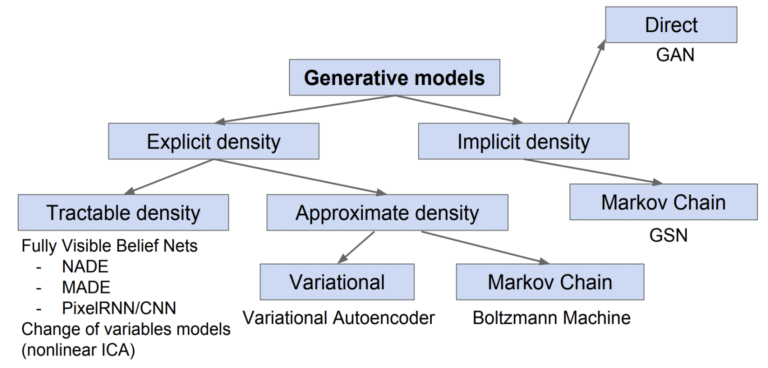
\includegraphics[width=0.48\textwidth]{Taxonomy.png}
\caption{Taxonomy of generative models: Ian Goodfellow}
\label{fig:tax}
\end{figure}

The most important distinction in models is the explicit density estimators vs
the implicit density estimators. In the former case these models explicitly
learn the density function of the dataset. That is, they learn by maximizing the
likelihood function, typically the log-likelihood, as defined by
Equation~\ref{eq:like}. 

\begin{equation}
    L(\theta|x) = \prod f(x_i|\theta)
    \label{eq:like}
\end{equation}

Implicit density estimators do not learn the likelihood
function and just learn a stochastic procedure that directly generates data.
This means that these different methods have different uses. For example, a
implicit method is not going to be well suited for understanding the bias in a
dataset because it is not learning the density function of that dataset. The
implicit method will typically have an advantage in being easier to train and
being more tractable. Unfortunately many problems are not tractable and thus
even explicit methods typically use approximate density estimations. We will
first discuss implicit density estimators and then explicit. In
section~\ref{sec:GAN} we will further discuss Generative Adversarial Networks
and how they work. In sections~\ref{sec:autoencoder} and \ref{sec:vae} we will
discuss autoencoders and variational autoencoders, which are approximate density
estimators. Finally, in section~\ref{sec:nf} we will discuss Normalizing Flows,
which are tractable density estimators.

\section{Generative Adversarial Networks}\label{sec:GAN}
Generative Adversarial Networks (GANs) are a type of generative model
that uses a minimax algorithm to generate images. The network is composed of
multiple parts: a generator and a discriminator, as shown in
Figure~\ref{fig:gan}. The generator takes as input some noise from a known
distribution and then the generator upscales that into the size of the desired
data while also trying to match the data. The discriminator takes two different
types of inputs and tries to distinguish between the two, real data as well as
data from the generator.

\begin{figure}[ht]
    \centering
    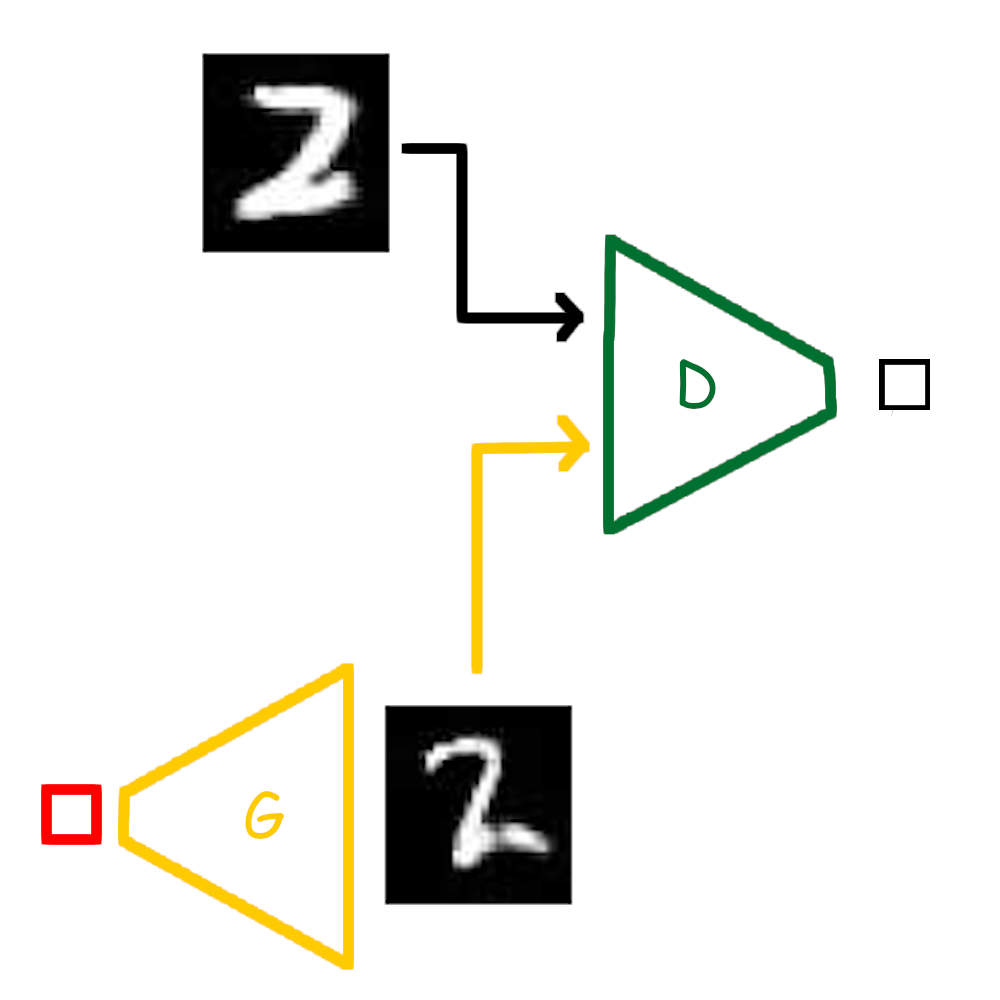
\includegraphics[width=0.48\textwidth]{GAN.png}
    \caption{A Generative Network where G represents the generator and D represents
        the discriminator.}
    \label{fig:gan}
\end{figure}

To train this network one trains the discriminator first, then the generator,
and then repeats the process. The goal is to make sure that the discriminator
can easily tell the difference between real and generated images. Then the
generator needs to be trained up to the point where it can fool the
discriminator. By doing this dual cycle eventually the generated data become so
good that the discriminator cannot be further improved by training. 

GANs are extremely popular in generative research because their ability to
produce high quality images. But because they are implicit density estimators
they have a few limitations. Because they do not learn the density function it
is more difficult to infer between different images, for example: someone
wearing glasses and someone not. Being able to infer this allows one to augment
an image to add the new feature. While there is plenty of research where people
have figured out how to solve these types of problems with GANs they do
not perform this action by direct inference like explicit density estimators do.
By looking at the latent space of a typical GAN, Figure~\ref{fig:ganLS}, we can
see that there is not a clear clustering of like features.

\begin{figure}[ht]
\centering
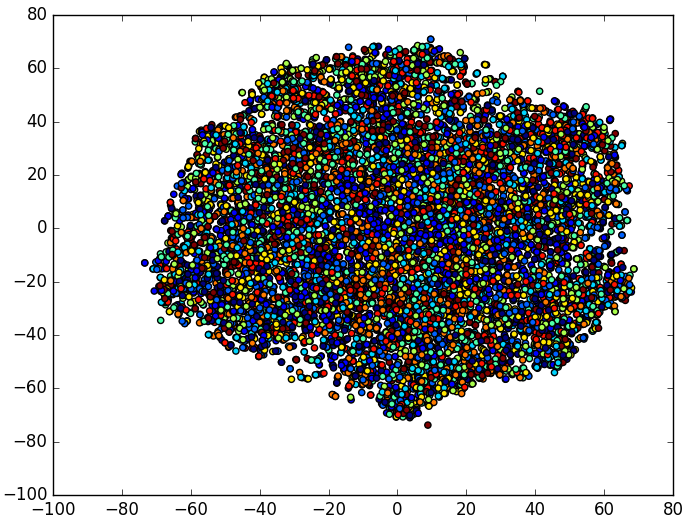
\includegraphics[width=0.48\textwidth]{GANLatent.png}
\caption{Latent space of a typical GAN}
\label{fig:ganLS}
\end{figure}

%\subsection{ClusterGAN}
%ClusterGAN~\cite{} tries to solve the problem of poor interpretability in the latent
%space. By doing this, ClusterGAN can allow GANs to perform a version of
%representation learning, or allowing the model to disentangle hidden features
%and semantics in the data. To accomplish this they use a mixture of discrete and
%continuous latent variables, use a novel backpropagation algorithm, and a
%clustering specific loss function. 
%
%For the discrete and continuous mixture of data they sample from normal random
%variables as well as one-hot encoded vectors. By modifying the standard
%deviation they can ensure that the latent space separates. 
%
%\textbf{TODO}

\subsection{StyleGAN}
StyleGAN is a popular state of the art GAN architecture that produces
impressively good images. One of the drawbacks of GANs is that they frequently
have "monsters", blobs, and phase errors. An example of the blobs is shown in
Figure~\ref{fig:blobs}. GAN monsters are grotesque looking creations that
generally take on features like the intended but with extra features. For
example a GAN generated cat may have a head disassociated from its body or a GAN
face could have a mouth where an eye should be. The third type of problem they
solved is a phasing issue. A common example of this is how teeth will align
forward while a head may be looking in a different direction.

\begin{figure}[ht]
\centering
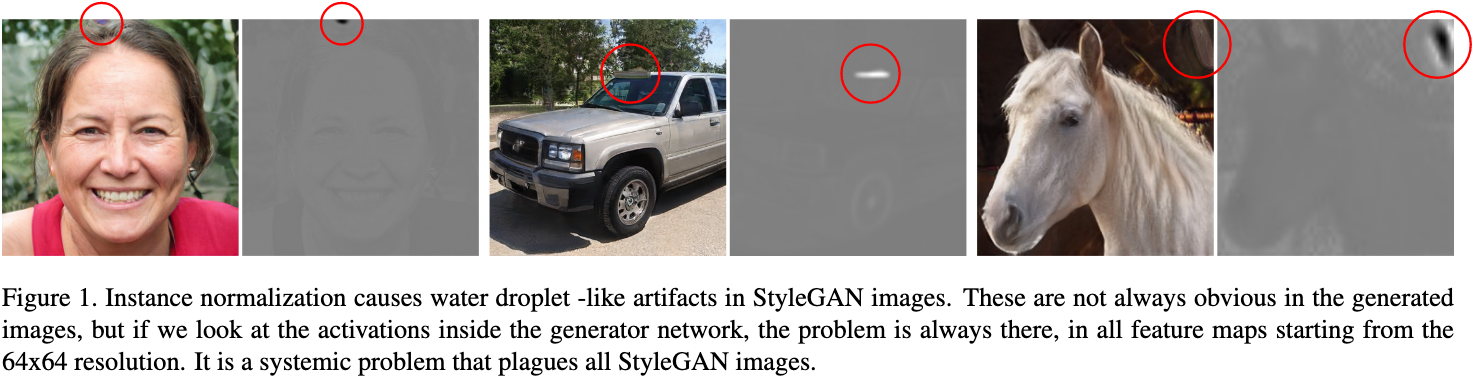
\includegraphics[width=0.48\textwidth]{StyleGAN2_blobs.png}
\caption{GAN blobs from StyleGAN}
\label{fig:blobs}
\end{figure}

StyleGAN2~\cite{Karras2019stylegan2} solves this problem with a few changes to their original work. To
reduce the instances of monsters they introduced a perceptual path length (PPL)
regularizer. They introduced this because they noticed that images with higher
quality had lower PPL scores. By introducing this regularizer they can ensure
that the generated images will have minimized PPL. In a change of pace from
conventional GAN architectures, StyleGAN2 used skip generators and a residual
discriminator to replace progressive growing. They also introduced lazy
regularization, where they split the loss and regularization terms, and they
regularize every 16 minibatches. Finally, StyleGAN2 doubled the size of the
output images, to 1024x1024, greatly increasing the resolution of generated
images. With all these improvements StyleGAN2 was able to generate unprecedented
high quality images, improving as much as 30\% from StyleGAN, a work done only a
year earlier. 

\section{AutoEncoders}\label{sec:autoencoder}
Autoencoders are a form of explicit density estimators. In essence an
autoencoder tries to learn a latent space that can regenerate the images that it
takes as input. Once the network has been sufficiently trained the network can
recreate samples from the original dataset. Figure~\ref{fig:ae} shows the
general form of an autoencoder.

\begin{figure}[ht]
\centering
\includegraphics[width=0.48\textwidth]{autoencoder.png}
\caption{Autoencoder architecture}
\label{fig:ae}
\end{figure}

More formally an autoencoder seeks to map a sample $x$ to a latent variable $z$
where $x\in\mathbb{R}^n$ and $z\in\mathbb{R}^m$ and $n<m$. An autoencoder is a
one of the most simple architectures because we can simply take the mean square
error (MSE) between the generated image and the one trained on, making the
autoencoder an unsupervised learner. The encoding section of the network is only
needed for training. The drawback of the autoencoders is that they can not
generate new and unique samples. 

\section{Variational AutoEncoders}\label{sec:vae}
The Variational Autoencoder (VAE) is a small twist on autoencoder that allows
for a variation on data, allowing for the generation of unique samples. The
problem is that we want to learn the conditional probability 
$p(z|x) =\frac{p(x|z)p(z)}{p(x)}$ but $p(x) = \int p(x|z)p(z)dz$ is often
intractable. Instead a VAE learns an approximate function $q(z|x)$ that is
tractable. Because this function is different we need to introduce the
Kullback-Leibler (KL) divergence~\ref{eq:kl} to the regularization function, in
addition to the MSE. Additionally VAEs use a reparamerization trick because we
cannot backprop through stochastic nodes. To do this $\mu$ adn $\sigma$ are held
constant and $z$ becomes $z=\mu + \sigma\odot\epsilon$ and $\epsilon$ is allowed
to vary.

\begin{equation}
D_{KL}(P||Q) = \int P(x)\log\left(\frac{P(x)}{Q(x)}\right)dx
\label{eg:kl}
\end{equation}

By making these additions to the autoencoder the VAE is able to generate
variational data and actually learn the density of the dataset. An example of
the VAE architecture is shown in Figure~\ref{fig:vae}.

\begin{figure}[ht]
\centering
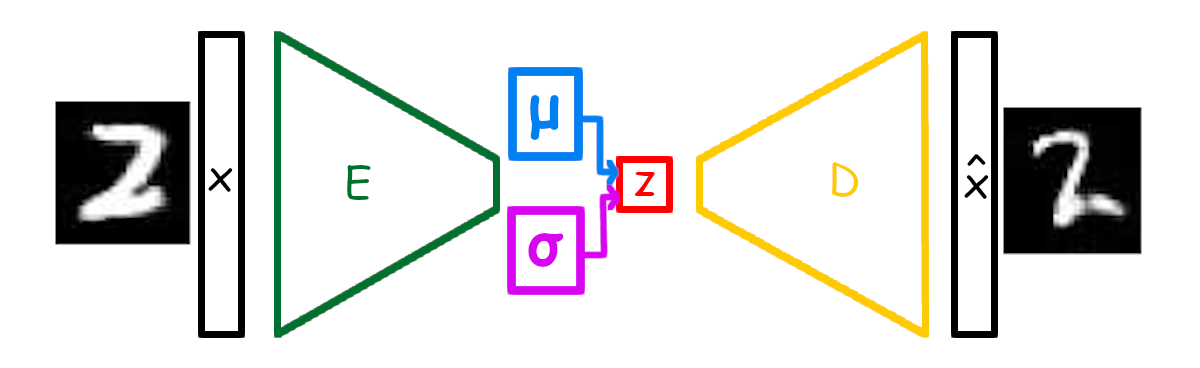
\includegraphics[width=0.48\textwidth]{VAE.png}
\caption{Autoencoder architecture}
\label{fig:vae}
\end{figure}

\section{Normalizing Flows}\label{sec:nf}
Normalizing Flows are an explicit density function that learns a tractable
density. To do this Flows use the change of variable methods to learn a
tractable density function that can be learned and use the change of variable
method~\ref{eq:cov} to map to the intractable density function. 

\begin{equation}
p(x) = q(f^{-1}(x))|det\frac{df^{-1}(x)}{dx}|
\label{eq:cov}
\end{equation}

The change of variable method works because the integral of all probability
density functions is 1 ($\int p(x)dx = \int q(z)dz = 1$). Through this
Flows are composed of a series of bijective functions, that is functions that
are one-to-one and onto another data space. This is shown in
Figure~\ref{fig:nf}.

\begin{figure}[ht]
\centering
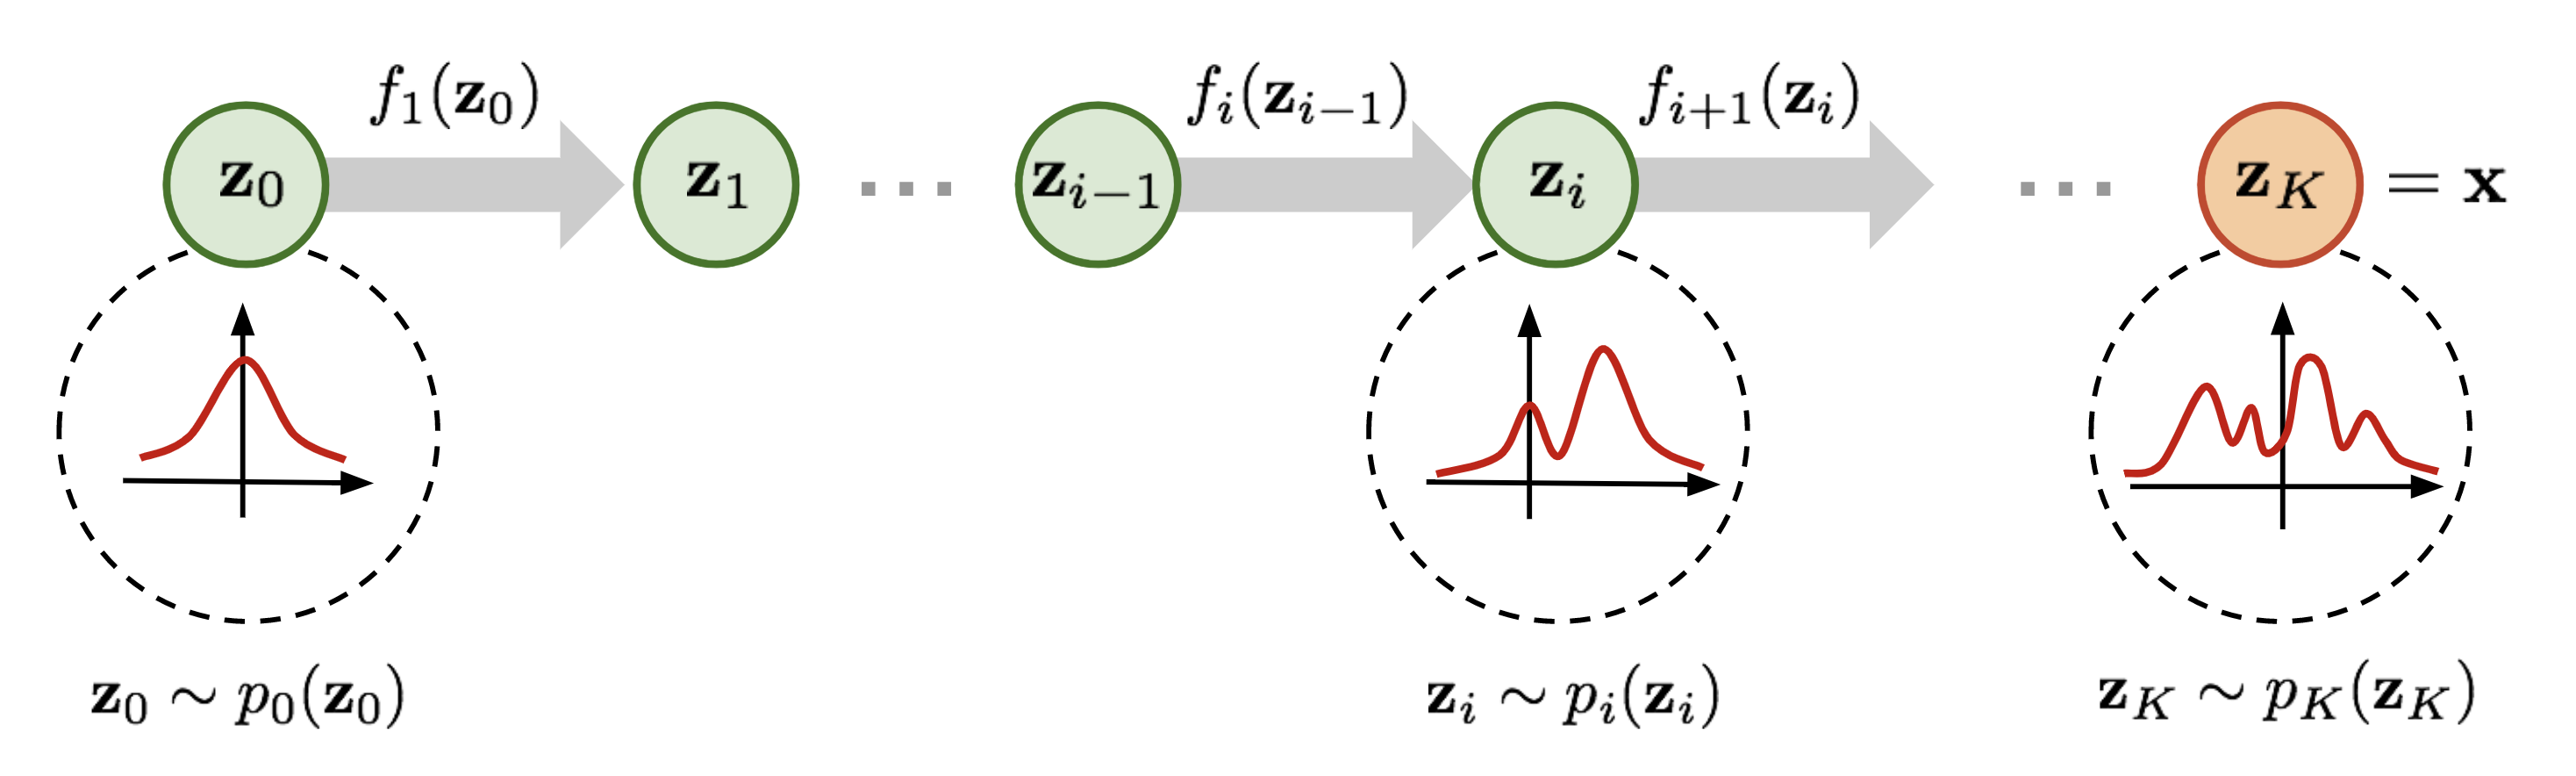
\includegraphics[width=0.48\textwidth]{normalizing-flow.png}
\caption{Architecture of a normalizing flow}
\label{fig:nf}
\end{figure}

Normalizing flows are bidirectional models, in that they are trained in both
directions. Because of the bijective nature of these networks one samples from
the tractable distribution and the input data and send them backwards through
the network. The loss function is then used to learn the difference between
these distributions. This makes flows unsupervised learners. 

\subsection{GLOW}
GLOW~\cite{GLOW} was the first normalizing flow that was able to generate realistic looking
images with larger datasets like CelebA. GLOW is based on two predecessors,
NICE~\cite{NICE} and RealNVP~\cite{RealNVP}, and essentially is a much larger version of
RealNVP with some minor changes. GLOW showed that like traditional deep neural
networks, normalizing flows could generate substantially better results by
deepening the network. The other major contribution that GLOW improves from
RealNVP is that GLOW uses a 1x1 invertible convolutional layer. The architecture
of GLOW is shown in Figure~\ref{fig:glow}.

\begin{figure}[ht]
\centering
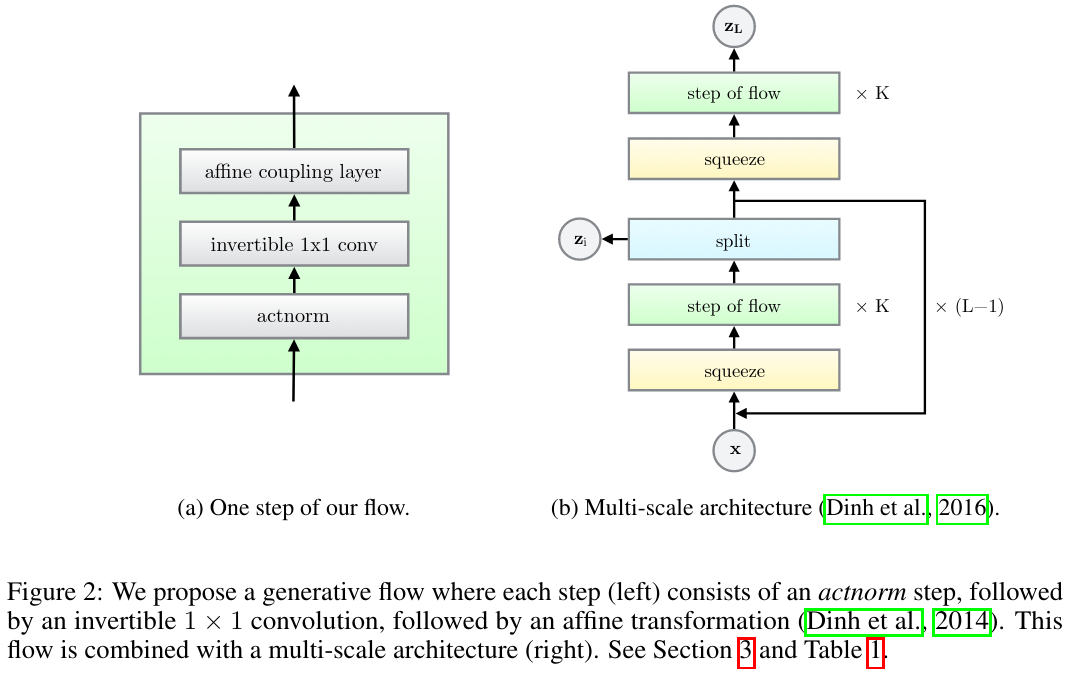
\includegraphics[width=0.48\textwidth]{GLOWModel.png}
\caption{Construction of GLOW}
\label{fig:glow}
\end{figure}

The key parts of this type of flow is that there is a multi-scale architecture
that is able to learn different scales of the data. This multi-scale
architecture allows the network to better learn fine detail in data and this
provides the higher resolution achieved by this network. The larger the data
being trained on, the more layers are needed for accurately reproducing data.
The major downside of flows is that they are substantially more difficult to
train than networks like VAEs or GANs. The advantage of these networks is that
they are able to learn the density, and thus it is trivial to infer between
different latent variables. For example, it is easy to introduce glasses on a
face by performing a linear interpolation between the image and the center of
images with glasses. The center of images with glasses can similarly be easily
found by taking the mean of several images that have glasses in them, requiring
one to know the feature that is being looked for.

\section{Conclusion}
In this survey we have seen some of the most popular types of generative models
and learned about some of their uses. Each form of generative model has
different advantages and disadvantages. We saw that GANs were great at producing
high quality and realistic images by directly learning how to generate images
and not concerning themselves with things like learning the likelihood of a
function. We saw that autoencoders and VAEs are simple to construct but are not
as powerful in their reconstructions. Lastly we saw how normalizing flows can be
used to learn the density function and in turn can be used to trivially infer
between different latent variables.



{\small
\bibliographystyle{ieee_fullname}
%\bibliography{egbib}
\bibliography{bibliography}
}

\end{document}

%   \url{http://www.pamitc.org/documents/mermin.pdf}.
%   \begin{quote}
%   \begin{center}
%       An analysis of the frobnicatable foo filter.
%   \end{center}
%   
%      In this paper we present a performance analysis of our
%      previous paper [1], and show it to be inferior to all
%      previously known methods.  Why the previous paper was
%      accepted without this analysis is beyond me.
%   
%      [1] Removed for blind review
%   \end{quote}
%   
%   
%   
%   \begin{quote}
%   \begin{center}
%        An analysis of the frobnicatable foo filter.
%   \end{center}
%   
%      In this paper we present a performance analysis of the
%      paper of Smith \etal [1], and show it to be inferior to
%      all previously known methods.  Why the previous paper
%      was accepted without this analysis is beyond me.
%   
%      [1] Smith, L and Jones, C. ``The frobnicatable foo
%      filter, a fundamental contribution to human knowledge''.
%      Nature 381(12), 1-213.
%   \end{quote}
%   
%   
%   \noindent
%   FAQ\medskip\\
%   {\bf Q:} Are acknowledgements OK?\\
%   {\bf A:} No.  Leave them for the final copy.\medskip\\
%   {\bf Q:} How do I cite my results reported in open challenges?
%   {\bf A:} To conform with the double blind review policy, you can report results of other challenge participants together with your results in your paper. For your results, however, you should not identify yourself and should not mention your participation in the challenge. Instead present your results referring to the method proposed in your paper and draw conclusions based on the experimental comparison to other results.\medskip\\
%   
%   \begin{figure}[t]
%   \begin{center}
%   \fbox{\rule{0pt}{2in} \rule{0.9\linewidth}{0pt}}
%      %\includegraphics[width=0.8\linewidth]{egfigure.eps}
%   \end{center}
%      \caption{Example of caption.  It is set in Roman so that mathematics
%      (always set in Roman: $B \sin A = A \sin B$) may be included without an
%      ugly clash.}
%   \label{fig:long}
%   \label{fig:onecol}
%   \end{figure}
%   
%   \begin{tabular}{ll}
%    \verb'$conf_a$' &  $conf_a$ \\
%    \verb'$\mathit{conf}_a$' & $\mathit{conf}_a$
%   \end{tabular}\\
%   
%   This is incorrect: ``... subsequently developed by Alpher \etal~\cite{Alpher03} ...''
%   
%   \begin{figure*}
%   \begin{center}
%   \fbox{\rule{0pt}{2in} \rule{.9\linewidth}{0pt}}
%   \end{center}
%      \caption{Example of a short caption, which should be centered.}
%   \label{fig:short}
%   \end{figure*}
%   \begin{verbatim}
%   \setcounter{page}{4321}
%   \end{verbatim}
%   where the number 4321 is your assigned starting page.
%   
%   
%   \begin{table}
%   \begin{center}
%   \begin{tabular}{|l|c|}
%   \hline
%   Method & Frobnability \\
%   \hline\hline
%   Theirs & Frumpy \\
%   Yours & Frobbly \\
%   Ours & Makes one's heart Frob\\
%   \hline
%   \end{tabular}
%   \end{center}
%   \caption{Results.   Ours is better.}
%   \end{table}
%   
